\section{Fysisk Lag}

\subsection{Mediet}
Transmissionsmediet der bruges til at sende data over er lyd i form af DTMF toner. Der findes 16 forskellige DTMF toner. Ud fra emperiske målinger er den hurtigste sendetid fastlagt til at være 25ms per tone for at en tone bliver afkodet på modtagersiden.

\subsection{SFML}
Til at afsende og optage lyd bruges der et bibliotek kaldet Simple and Fast Multimedie Library forkortet SFML. Dette bibliotek er skrevet i c++ og indeholder funktioner til at interagerer med hardwaren uden at skulle rode med at initialiserer og opsætte hardwaren. Biblioteket er opdelt i forskellige underbiblioteker alt efter, hvilken del af computerens hardware der skal interageres med. Og der kan derfor nøjes med kun at inkluderer den funktionalitet der er ønsket i projektet. Biblioteket er veldokumenteret på deres hjemmeside, hvor der også findes adskille tutorials til, hvordan de forskellige funktioner bruges.

\subsection{Transmitter}


\subsubsection{Kodning}
For at kunne sende data over mediet skal der vælges en linjekodning der fastsætter, hvor mange dataelementer der repræsenteres af et signalelement. Dataraten er det antal bits der kan sendes på et sekund og signalraten er det antal signalelementer der sendes på et sekund. Målet med linjekodningen er at øge dataraten og sænke signalraten. Da en øget datarate øger hastigheden af kommunikationen og en sænket signalrate sænker niveauet for båndbredde på mediet. Hvis en DTMF tone anses for at være et signalelement så vil der med et signalelement kunne opnås $16^{1}$ mulige kombinationer af signalelementer. 


\subsection{Receiver}

\subsubsection{Goertzel}

For at afgøre om bestemte frekvenser er til stede i et signal anvendes Goertzel-algoritmen. Den kan returnere en magnitude, hvis størrelse afhænger af hvor meget signalet man giver, korrelerer med bestemte frekvenser. På den måde kan man se på om den returnerede magnitude er over et bestemt threshold, for at afgøre om den ønskede frekvens er til stede i signalet.\\

For at konvertere fra frekvenser til frekvens-bins og  bruges følgende formler:

\noindent\begin{minipage}{.5\linewidth}
\begin{equation}
  k=N*\dfrac{targetFrekvens}{Samplerate}
\end{equation}
\end{minipage}%
\begin{minipage}{.5\linewidth}
\begin{equation}
  \omega = \dfrac{2*\pi}{N}*k
\end{equation}
\end{minipage}


Fordelen ved at anvende Goertzel-algoritmen frem for en DFT/FFT er, at man kan nøjes med kun at kigge på nogle få frekvens-bins ad gangen, og så derfra finde DFT-koefficienten for den bin alene. Den udregning er langt nemmere at foretage, så længe man kun er interesseret i relativt få frekvenser. Selve algoritmen kommer fra et 2. ordens IIR-båndpas-filter, med en pol og dens konjugerede placeret på enhedscirklen i de bins, hvor man leder efter frekvenser. En anden ting der taler for Goertzel-algoritmen i vores tilfælde, er at de tungeste udregninger kan foretages på forhånd, og gemmes som konstanter i en tabel, man så kan slå op i. I goertzel-klassen foretages det tunge arbejde i en initialiseringsfunktion \textit{init()}, der regner alle konstanter til hver frekvens og gemmer dem i et map, man så kan slå op i med den ønskede frekvens. For at lave udregningerne, skal man bare kende samplingfrekvensen og antallet af samples man regner med at bruge i selve algoritmen - det vil i vores tilfælde være sampleWindow. Der udregnes også en skaleringsfaktor, der skal ganges på DFT-koefficienten's magnitude for at finde det en-sidede amplitudespektrum. Amplitudespektret vil være den værdi, man kigger på for at afgøre om en frekvens er til stede i et signal. 
Overføringsfunktionen til Goertzel-filteret:



\begin{equation}\label{eq:transferfunction}
H(z) = \frac{1}{1-2Cos(\omega)z^{-1}+z^{-2}}
\end{equation}


I goertzel-klassen foretages det tunge arbejde i en initialiseringsfunktion \textit{init()}, der regner alle konstanter til hver frekvens og gemmer dem i et map, man så kan slå op i med den ønskede frekvens. For at lave udregningerne, skal man bare kende samplingfrekvensen og antallet af samples man regner med at bruge i selve algoritmen. Der udregnes også en skaleringsfaktor, der skal ganges på DFT-koefficienten's magnitude for at finde det en-sidede amplitudespektrum. Amplitudespektret vil være den værdi, man kigger på for at afgøre om en frekvens er til stede i et signal. \\
Når selve algoritmen bliver brugt, køres alle samples igennem filteret og derefter regnes magnitude ud, fra den reelle og den imaginære del af DFT-koefficienten.





\subsubsection{Recorder}

Recorderen kommer fra SFML-biblioteket. En af fordelene ved at bruge SFML, er at det ikke er nødvendigt at programmere interaktionen med mikrofoner og højtalere på et lavt niveau. SFML har indbyggede funktioner, der sørger for at oprette og vedligeholde forbindelse med eksterne enheder. Man har mulighed for at designe sin egen recorder-klasse, ved at arve fra en af de indbyggede klasse og så overloade tre funktioner der returnerer bools. Funktionerne bruges til at fortælle superklasserne om de kan fortsætte med at udføre bestemte handlinger, man sætter igang med andre funktioner. Hvis de returnerer false stoppes handlingen og omvendt hvis de returnerer true.

\begin{itemize}

\item \textbf{onStart():} Bliver kørt når man beder om at starte en optagelse. Her kan man indsætte forskellige tests der afgør om det er smart at fortsætte med at starte optagelsen. Det kunne eksempelvis testes, om der overhovedet kan skabes kontakt til en mikrofon.

\item \textbf{onProcessSamples():} Funktionen får givet en pointer til samples og antallet af dem som parametre. Det er så muligt at flytte dem til sin egen buffer til videre behandling. Den bliver kørt med jævne mellemrum, når en optagelse er startet, og mellemrummet kan defineres med funktionen setProcessingInterval(). 

\item \textbf{onStop():} Bliver kørt når man beder om at stoppe en optagelse.

\end{itemize}

Der er sådan set en fungerende optagerklasse inkluderet i SFML-biblioteket fra starten af, men den er lidt mindre fleksibel, og nærmere tiltænkt brug som en slags plug-and-play optager. Det er ikke muligt løbende at trække samples ud fra bufferen, hvis man er interesseret i at processere dem i real-time. Derfor er en custom recorder at foretrække i vores tilfælde. \\
Recorderen kører i sin egen tråd, parallelt med alt andet, så derfor skal man huske at låse delte ressourcer med en mutex, for at forhindre data race situationer - det er nødvendigt når man læser fra eller skriver til bufferen. SFML har også sin egen mutex-klasse som vi bruger flere steder.

\subsubsection{Analyzer}

Analyzer-klassen fungerer som bindeled mellem recorderen og goertzel-klassen. Det er den der styrer behandlingen af de samples der kommer ind. Den's primære opgave er at søge sin buffer igennem for frekvenser, der indgår i DTMF-toner. Hvis den finder nogen, oversættes de til karakterer, der kan sendes videre i systemet. Analyzeren har sin egen buffer, som den kan arbejde på i fred. Når denne buffer er tømt, kan der hentes nye samples ind fra recorderen's buffer. \\

Detektionen af DTMF-toner udføres af to funktioner - \textit{syncToFirstDTMF()} og \textit{findNextDTMF()}. De er designet ud fra den antagelse, at når der kommer beskeder ind, vil de altid komme i en strøm af toner adskilt af et lille mellemrum uden lyd. Så hvis man kan finde den første DTMF-tone i denne strøm, så kan man blive ved med at kigge på et antal samples frem i tiden, der svarer til længden af hver tone. Det kan nemt udregnes fra samplefrekvensen \eqref{eq:sampleWindow}. \\

\begin{equation}
sampleWindow=sampleRate[samples/s]*toneLaengde[s]
\label{eq:sampleWindow}
\end{equation}

\begin{figure}[h]
\centering
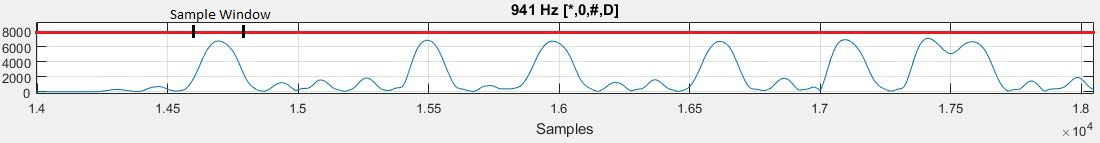
\includegraphics[scale=0.5]{Billeder/Samplewindow.PNG}
\caption{Her ses samplewindow, når det er stillet optimalt på den første tone. Magnitudes ved 941 Hz er vist op ad y-aksen}
\label{fig:Samplewindow}
\end{figure}
Når \textit{syncToFirstDTMF} leder bufferen igennem, er dens vigtigste opgave at stille sampleWindow mere eller mindre lige oveni den første DTMF-tone den finder, så magnitude på den næste gang samples er på sit højeste. På den måde kan \textit{findNextDTMF} blive ved med at kigge på et sampleWindow, finde tonen og så slette alle de analyserede samples fra bufferen uden at bekymre sig om, om man har slettet for meget af en anden tone. Inden den første tone er fundet, slettes der kun 1/4 af sampleWindow ad gangen, så man ikke risikere at slette nogle vigtige samples. Første gang man støder på en tone, søges et område á to sample vinduer i nærheden igennem, for at finde den position, hvor magnitude for den fundne karakter er størst. Den viden kan så bruges til at bestemme nogenlunde præcist, hvor mange samples der skal slettes, for at det næste vindue står lige oveni en tone. På transmittersiden, er der sørget for at volumen er højest midt i en tone ved at gange et slags vindue på - på den måde kan man godt antage, at magnitude fra goertzel-algoritmen er højest cirka midt i tonen.

\subsubsection{Physical Receive}

PhysicalReceive-klassen har til opgave at styre hvordan hele analyseringsprocessen forløber, og så i sidste ende sende en vektor med bools op til datalink-laget til videre behandling. Da denne klasse er forbindelsen til de øvre lag, er der her lavet funktioner til at starte og stoppe recorderen. Funktionen \textit{continuousAnalysis()} kan køre i sin egen tråd, og sørger for at bufferen i Analyzer-klassen løbende bliver kigget igennem for DTMF-toner. Til styringen af analyzeren, er der to vigtige ting at holde øje med.

\begin{itemize}

\item \textbf{Hvornår bliver strømmen af toner brudt.} Lige så snart der ikke kan findes flere toner sættes en bool, \textit{charStringBroken}, der fortæller Analyzeren at den er nødt til at synkronisere igen. Så længe denne bool ikke er sat, fortsætter Analyzeren med at kigge på samples en gang, returnere den fundne tone og så slette dem igen. 
\item \textbf{Hvornår er bufferen ved at være tømt.} Når bufferen når under en størrelse af 4 samplewindows, må der ikke foretages mere, før der er fyldt nye samples i fra recorderen. På den måde bryder man ikke den synkronisering, der er lavet en gang, og det forhindrer også funktionen i at forsøge at indeksere uden for bufferen.
\end{itemize}

De to første toner i en hvilken som helst sammenhængende strøm bliver ignoreret, da det altid vil være en preamble. Preamblen er lavet for at gøre synkroniseringen nemmere. Vi valgte DTMF-tonerne 'A' og '6' da de ikke har nogen overlappende frekvenser - tests vi lavede viste, at magnitude for en frekvens, der fandtes i to toner lige ved siden af hinanden, ikke faldt ret meget imellem tonerne. Det havde den effekt at sampleWindow kunne stå forkert selv efter synkroniseringen. Problemet er sidenhen blevet gjort mindre af at gange et Hann-Window på samples i goertzel-algoritmen, men preamblen bliver stadig brugt. Se reference her!!

\begin{figure}[h]
\centering
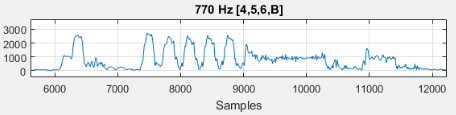
\includegraphics[scale=0.8]{Billeder/NoWindow.PNG}
\caption{Her ses magnitude på 697 Hz for et signal sendt med en tonelængde på 20 ms, uden en vinduefunktion på modtagersiden}
\label{fig:NoWindow}
\end{figure}

\begin{figure}[h]
\centering
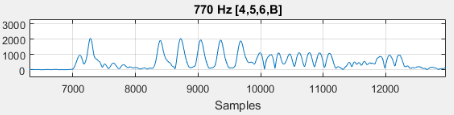
\includegraphics[scale=0.8]{Billeder/HannWindow.PNG}
\caption{Her ses magnitude på 697 Hz for samme signal sendt med en tonelængde på 20 ms, med et Hann-vindue på modtagersiden}
\label{fig:NoWindow}
\end{figure}


Alle toner der ikke er en del af preamblen, bliver konverteret til bools og placeret i en vektor, \textit{boolsReceived}, der fungerer som bindeledet imellem det fysiske, og datalinklaget. I kraft af at de to lag kører i hver sin tråd er det nødvendigt at låse \textit{boolsReceived} med en mutex, for at forhindre data race situationer. Det gøres i praksis ved at låse funktionerne \textit{addNibble()} og \textit{extractBools()}, der henholdsvis skriver til og læser fra vektoren. Datalink-laget trækker selv bools fra det fysiske lag, når det er klart til det.\\

